The sensitivity analysis represents how sensitive the model is to the variation in the value of the variables. The following section explains the effect of the sensitivity analysis on the three initiatives with the best outcomes. The exogenous variables being looked into are "weight of quality on behavior", "weight of attitude on behavior" and "weight of costs on attitude". The simulation focuses on the material recycling percentage in scenarios where the values of the variables are 50\% lower and 50\% higher. 

\indent \newline
When running the simulations, it is clear that the scenarios react in the same pattern. None of the given scenarios regarding the suggested initiatives results in a reduced material recycling percentage.

\begin{table}[H]
\centering
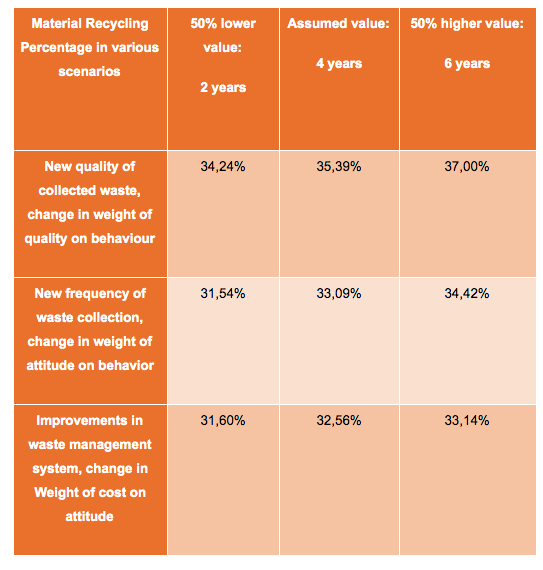
\includegraphics [scale=0.50,angle=360]{tables/scenarios.png}
\caption{Material Recycling Percentage in Different Scenarios}
\label{tbl:scenarios}
\end{table}

\indent \newline
The recommendations from the previous chapter still stands. As measured in the table above, one can clearly state that the new quality of collected waste has the best results in every scenario. For better visualization, please see figures 6.1, 6.2 and 6.3. These figures represent the top three initiatives separately simulated with various values from the exogenous variables at different time slots. 

\indent \newline
Regarding the new quality of collected waste initiative, it has an impact on the material recycle percentage, which makes it interesting to apply a sensitivity analysis. The sensitivity analysis reveals that this initiative is sensitive to a change in the exogenous variable "weight of quality on behavior". Furthermore, the analysis reveals that the model behaves as expected and that it reflects the real world. When increasing the number of waste containers, it should result in a higher material recycling percentage, which is projected in the sensitivity analysis. The initiative "new frequency of waste collection" follows the same pattern as the previous initiative. It is sensitive to an increase in the exogenous variable "weight of attitude on behavior". The third initiative which is reflected through "improvements in waste management system" is also sensitive to the correlated exogenous variable "weight of costs on attitude". It was expected to be sensitive to change, because if Oslo municipality increases the investments, the material recycling percentage will increase as well. 

\indent \newline
The sensitivity analysis shows that adjusting the values related to the exogenous variables and the time-intervals does not change the initial recommendations. The third scenario isn't as sensitive as the previous two initiatives, but still sensitive to some degree. 

\begin{figure}[H]
\centering
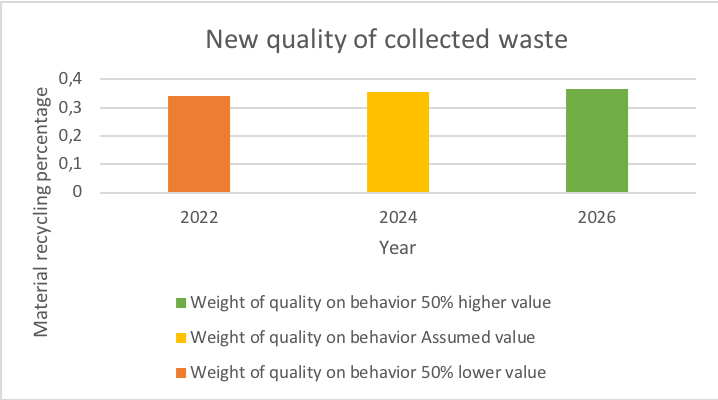
\includegraphics [scale=0.80,angle=360]{figures/sensitivitynew.png}
\caption{Sensitivity Result For New Quality of Collected Waste}
\label{fig:sensitivitynew}
\end{figure}

\begin{figure}[H]
\centering
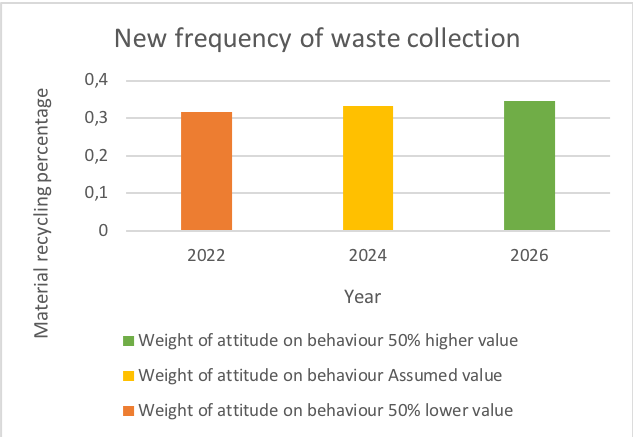
\includegraphics [scale=0.80,angle=360]{figures/sensitivitynewf.png}
\caption{Sensitivity Result For New Frequency of Waste Collection}
\label{fig:sensitivitynewf}
\end{figure}

\begin{figure}[H]
\centering
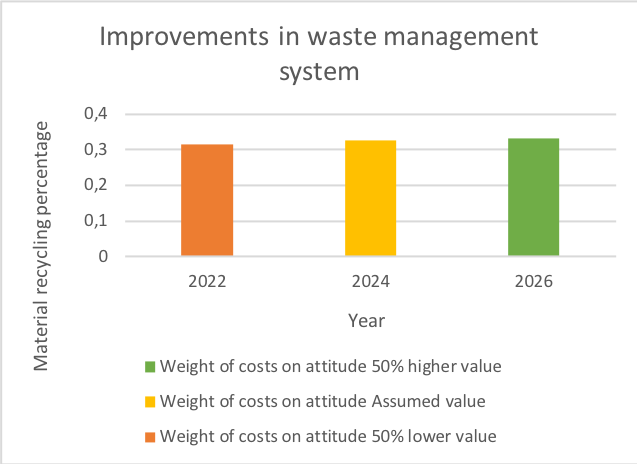
\includegraphics [scale=0.80,angle=360]{figures/sensitivityi.png}
\caption{Sensitivity Result For Improvements in Waste Management System}
\label{fig:sensitivityi}
\end{figure}